\section{Méthode de developpement}


\subsection{Cycle Itératif}
La méthode de développement pour le projet tuteuré est plus ou moins imposée. En effet pour pouvoir suivre l'avancement du projet, les tuteurs demandent aux étudiants d'utiliser un cycle itératif (figure \ref{cycle_iteratif}).

\begin{figure}[H]
\centering
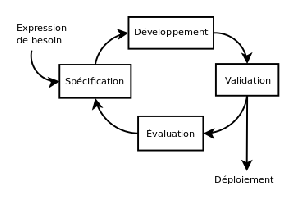
\includegraphics[width=8cm]{images/activite/cycle_iteratif.eps}
\caption{Schéma cycle Itératif}
\label{cycle_iteratif}
\end{figure}

\subsection{Outils de developpement}
Le choix du langage à utiliser était libre, nous avons donc opté pour un langage simple d'utilisation et ayant déjà fait ses preuves : \textbf{Java} (figure \ref{java_logo}).
\\
\\
\\

\begin{figure}[!h]
\centering

\includegraphics[width=8cm]{images/activite/javaLogo.eps}
\caption{Logo Java}
\label{java_logo}
\end{figure}


Nous avons choisi de travailler avec le logiciel \textbf{Éclipse} (figure \ref{eclipse_logo}), l'\gls{IDE} par excellence pour développer du \textbf{Java}.

\begin{figure}[H]
\centering

\includegraphics[width=8cm]{images/activite/eclipseLogo.eps}
\caption{Logo Éclipse}
\label{eclipse_logo}
\end{figure}

\textbf{Éclipse} est agréable à utiliser, il est libre de droits et fait partit des IDE les plus puissants de nos jours.
La bibliothèque nous permettant de faire des \gls{ihm} est swing, une bibliothèque native de Java, constamment mise à jours et très utilisée (donc très documenté).

\section{Planification}
Le projet a été découpé en sept itérations de durée variante (d'une semaine à un mois) en fonction des périodes d'examens et de vacances. Au cours de chaque itérations, de nombreux refactorings de code ainsi que d'organisation du code ont eu lieu.


\subsection{Itération 1 - 14/11/2016}

\subsubsection{Fonctionnalités et travail réalisé}
\begin{itemize}
\item Connexion à une base de données Oracle.
\item Mode requêtes SQL.
\end{itemize}

\subsubsection{Résultat}
L'utilisateur peut connecter à une base de données mais il y a des problèmes au niveau des champs de saisies. Le mode requête SQL ne fonctionne pas parfaitement.
Cette itération n'avait pas de grosse valeur pour le client. Elle a surtout permis de poser les bases de notre travail en groupe sur le projet en commençant à utiliser et se familiariser avec les outils de collaboration.


\subsection{Itération 2 - 02/12/2016}
\subsubsection{Fonctionnalités et travail réalisé}
\begin{itemize}
\item Correction des bugs sur la fenêtre de connexion et sur le mode Requêtes SQL.
\item Création de tables.
\end{itemize}

\subsubsection{Résultat}
Les bugs signalés sont corrigés et la vue de création de table fonctionne avec quelques bugs mineurs.
Cette itération fut satisfaisante pour le groupe car les attentes ont été respectées.

\subsection{Itération 3 - 15/12/2016}
\subsubsection{Fonctionnalités et travail réalisé}
\begin{itemize}
\item Connexion à MySQL.
\item Correction des bugs sur la fenêtre de création de tables.
\item Suppression de tables.
\item Modification de tables.
\end{itemize}

\subsubsection{Résultat}
Les bugs signalés sont corrigés et la vue de suppression de table fonctionne.
La modification de table ne fonctionne pas totalement.
Cette itération fut mitigée car la valeur apportée au client n'était pas conséquente. 


\subsection{Itération 4 - 12/01/2017}
\subsubsection{Fonctionnalités et travail réalisé}
\begin{itemize}
\item Correction de bugs sur la fenêtre de modification des tables.
\item CRUD des tuples d'une table.
\end{itemize}

\subsubsection{Résultat}
La fenêtre CRUD fonctionne partiellement (fonctionnalité update pas implantée) et quelques bugs sur l'insertion. 
La modification de table ne fonctionne pas totalement.
Cette itération fut peu satisfaisante mais a permis une remise en question de notre organisation. 

\subsection{Itération 5 - 02/02/2017}
\subsubsection{Fonctionnalités et travail réalisé}
\begin{itemize}
\item Correction des bugs sur le CRUD et ajout de la fonctionnalité update.
\item Début de la refonte des classes métiers de l'application.
\end{itemize}

\subsubsection{Résultat}
La fenêtre CRUD fonctionne avec quelques bugs mineurs.
La refonte des classes métiers avait pour but de stocker les différentes informations des tables de notre base de données et ainsi facilité l'accès à celles-ci.
La modification de table ne marche plus, mais la refonte des classes métiers va permettre de la faire fonctionner.
Cette itération fut satisfaisante car la refonte des classes métiers nous simplifie beaucoup de choses. 

\subsection{Itération 6 - 09/02/2017}
\subsubsection{Fonctionnalités et travail réalisé}
\begin{itemize}
\item Correction des bugs sur la fenêtre CRUD.
\item Fin de la refonte des classes métiers de l'application.
\item Modification des vues de Creation-Supression-Modification de tables pour qu'elles collent aux classes métiers.
\item Création et supression de contraintes (uniques et clées étrangères).
\end{itemize}

\subsubsection{Résultat}
La fenêtre CRUD fonctionne avec quelques bugs mineurs.
La création et la suppression de tables fonctionnent avec les nouvelles classes métiers.
La création et la suppression de contraintes ne fonctionne pas totalement.
Cette itération était dans la continuité de l'itération 6. 

\subsection{Itération 7 - 20/02/2017}
\subsubsection{Fonctionnalités et travail réalisé}
\begin{itemize}
\item Correction des bugs sur la création et la suppression de contraintes ainsi que sur la fenêtre CRUD.
\item Faire des requêtes graphiques (QBE).
\item Modification de tables.
\item Refactoring.
\end{itemize}

\subsubsection{Résultat}

La modification de tables et le QBE fonctionnent.
La création et la suppression de contraintes fonctionne avec quelques bugs mineurs.
Cette itération était surtout de la correction de bugs et de la rédaction du rapport. 


\section{Outils de collaboration}

\subsection{Gestionnaire de version}
Les premiers échanges que nous avons eus après l'attribution du sujet se sont concentrés sur le choix du gestionnaire de version que nous allions utiliser au cours du projet. Ce gestionnaire de version permet en autre de :
\begin{itemize}
\item Partager le code source de l'application.
\item Gérer des conflits lors de la modification simultanée d'un fichier.
\item Maintenir l'ensemble des versions d'un ou plusieurs fichiers.\\
\end{itemize}

Etant majoritairement habitué à utiliser Git, c'est vers un dép\^ot \textbf{Github} (figure \ref{github_logo}) que nous nous sommes tourné.

\begin{figure}[H]
\centering

\includegraphics[width=8cm]{images/activite/githubLogo.eps}
\caption{Logo GitHub}
\label{github_logo}
\end{figure}



\subsection{Répartition des tâches}
Au cours de leurs formations antérieures, certain membres du projet ont eu l'habitude d'utiliser l'outil de gestion de projet \textbf{Trello} (figure \ref{trello_logo}). C'est pourquoi nous avons utiliser cet outil pour répartir les tâches.\\

\begin{figure}[H]
\centering

\includegraphics[width=8cm]{images/activite/trelloLogo.eps}
\caption{Logo Trello}
\label{trello_logo}
\end{figure}

\textbf{Trello} permet de découper en <Tickets> les différentes t\^aches à réaliser. Ces tickets peuvent \^etres déplacés par les membres du projet dans différentes catégories :

\begin{itemize}
\item \textbf{TODO} - les t\^aches qu'il restent à faire. 
\item \textbf{DOING} - les \^aches en cours de développement.
\item \textbf{DONE} - les t\^aches qui sont terminées.
\item \textbf{TESTS} - les t\^aches qui sont validées et testées.\\
\end{itemize}

Chaque membre choisi un ticket dans la partie TODO et le déplace dans DOING. Puis lorsqu'il a terminé de dévelloper la fonctionnalité dans DONE et pour finir dans TEST.



\subsection{Communication}
Les outils de communication ont évolué au cours du projet. Nous avons tout d'abord utilisé naturellement la messagerie instantanée que propose \textbf{Facebook}. Cette messagerie simple, permet de partager des images ainsi que des documents.
Cependant nous souhaitions pouvoir discuter à l'oral ce que ne permet pas facilement la messagerie de Facebook. C'est pour cette raison que nous avons migré sur le logiciel \textbf{Discord}(figure \ref{discord_logo}) qui permet, en plus de la messagerie et de l'échange de documents, de discuter à l'oral ce qui a grandement facilité notre communication.

\begin{figure}[!h]
\centering

\includegraphics[width=10cm]{./images/activite/discordLogo.eps}
\caption{Logo Discord}
\label{discord_logo}
\end{figure}

De plus, nous avons installé un BOT sur le Discord, lié a GitHub, qui écrit un message lors d'une modification du dép\^ot git (figure \ref{bot_discord}).

\begin{figure}[!h]
\centering
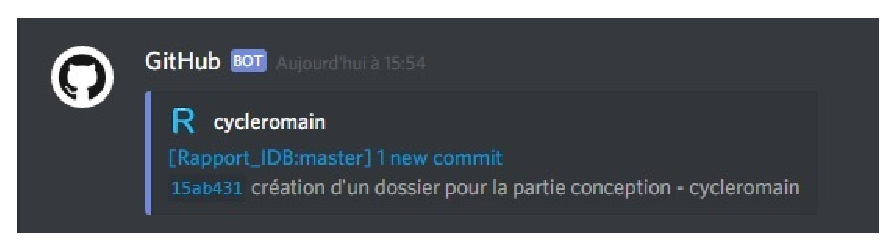
\includegraphics[width=10cm]{./images/activite/bot_discord.eps}
\caption{Message du BOT Discord lié à GitHub}
\label{bot_discord}
\end{figure}



\subsection{Partage de documents}
Tout au long du projet, nous avons produits différents documents qu'il nous a fallu stocker dans un endroit facile d'accès pour tous. Nous avons donc créé un dossier sur un \textbf{Google Drive} (figure \ref{googledrive_logo}) et l'avons partagé aux membres du groupe. Ce Drive nous a permis d'échanger et stocker des diagrammes, des pdfs, des documents texte, des maquettes pour les \glspl{ihm}* ainsi que d'autres fichiers que nous voulions conserver.

\begin{figure}[!h]
\centering

\includegraphics[width=10cm]{./images/activite/googleDriveLogo.eps}
\caption{Logo Google Drive}
\label{googledrive_logo}
\end{figure}



